\chapter{Typographie et communication visuelle}

\noindent
\textit{Dans les chapitres précédents, nous avons étudié les fondements du design graphique : sa définition, son histoire, son rôle, ses domaines, ses missions, puis les principes fondamentaux de la composition, et enfin la théorie des couleurs. Nous avons vu que la composition organise les éléments visuels et que la couleur leur donne une dimension émotionnelle et symbolique. Mais parmi ces éléments, il en est un qui occupe une place à part : la typographie.}

\vspace{1em}

\noindent
La typographie est bien plus qu'un simple habillage du texte : c'est le \terme{support premier du message verbal}. Dans la plupart des compositions graphiques, c'est le texte qui porte l'information essentielle : un titre, un slogan, une marque, une date, un mode d'emploi. Sans typographie, le message verbal est illisible. Avec une mauvaise typographie, il est confus, désagréable, voire incompréhensible. Avec une bonne typographie, il est clair, élégant, mémorable.

\vspace{1em}

\noindent
Ce chapitre a pour objectif de te donner les connaissances théoriques et les compétences pratiques nécessaires pour maîtriser la typographie. Nous commencerons par définir ce qu'est la typographie et retracer son histoire. Nous étudierons ensuite l'anatomie des caractères, les grandes familles de polices, les règles de lisibilité, les unités typographiques, les techniques d'espacement, l'association des polices, la hiérarchie typographique, et enfin les erreurs à éviter. À la fin de ce chapitre, tu sauras choisir, associer et mettre en page des typographies professionnelles.

% ============================================================
\section{Définition et histoire de la typographie}
% ============================================================

\subsection{Qu'est-ce que la typographie ?}

\begin{quote}
\textbf{La typographie est l'art et la technique de la composition des textes, comprenant le choix des caractères, leur disposition, leur espacement et leur mise en page, en vue de produire un message lisible, esthétique et expressif.}
\end{quote}

Cette définition mérite d'être décomposée.

\subsubsection{Un art et une technique}

La typographie est à la fois un \terme{art} (elle fait appel au goût, à la sensibilité, à la créativité) et une \terme{technique} (elle repose sur des règles, des mesures, des conventions). Un bon typographe est celui qui maîtrise les deux dimensions.

\subsubsection{La composition des textes}

La typographie ne se limite pas au choix d'une police : elle englobe la \terme{composition} du texte, c'est-à-dire l'organisation de tous ses paramètres :

\begin{itemize}
    \item Le \terme{choix des caractères} (police, graisse, style).
    \item La \terme{taille} des caractères.
    \item L'\terme{espacement} entre les lettres, les mots, les lignes.
    \item L'\terme{alignement} du texte.
    \item La \terme{hiérarchie} entre les différents niveaux de texte.
    \item La \terme{mise en page} dans un format donné.
\end{itemize}

\subsubsection{Un message lisible, esthétique et expressif}

La typographie vise trois objectifs complémentaires :

\begin{itemize}
    \item \terme{Lisibilité} : le texte doit être facile à lire.
    \item \terme{Esthétique} : le texte doit être agréable à regarder.
    \item \terme{Expressivité} : le texte doit transmettre une intention, une ambiance, une identité.
\end{itemize}

Une typographie réussie est celle qui atteint ces trois objectifs simultanément.

\subsection{Pourquoi la typographie est-elle essentielle ?}

La typographie est essentielle pour plusieurs raisons.

\subsubsection{Elle porte le message verbal}

Dans la plupart des compositions graphiques, le texte est le support principal de l'information. Sans typographie lisible, le message est perdu.

\subsubsection{Elle structure la composition}

La typographie crée des blocs, des hiérarchies, des rythmes. Elle organise la composition autant que les images.

\subsubsection{Elle transmet une identité}

Une typographie particulière peut identifier une marque, un journal, une époque. Pense à la typographie de \emph{The New York Times}, à celle de Coca-Cola, à celle de Google.

\subsubsection{Elle crée une émotion}

La typographie suscite des émotions : élégance, modernité, tradition, audace, douceur. Elle participe à l'ambiance générale de la composition.

\subsection{Brève histoire de la typographie}

\subsubsection{L'Antiquité}

Les premières formes de typographie apparaissent dans l'Antiquité :

\begin{itemize}
    \item Les \terme{hiéroglyphes} égyptiens (vers 3200 av. J.-C.).
    \item L'\terme{écriture cunéiforme} mésopotamienne.
    \item L'\terme{alphabet phénicien} (vers 1050 av. J.-C.).
    \item L'\terme{alphabet grec} (vers 800 av. J.-C.).
    \item L'\terme{alphabet latin} (vers 700 av. J.-C.).
\end{itemize}

Les Romains gravent dans la pierre des inscriptions dont les proportions sont soigneusement étudiées. La \terme{colonne Trajane} (113 apr. J.-C.) est un exemple célèbre : ses caractères, appelés \terme{capitales romaines}, ont inspiré les caractères à empattements modernes.

\subsubsection{Le Moyen Âge}

Au Moyen Âge, les moines copistes produisent des \terme{manuscrits enluminés} où le texte, les lettrines, les bordures et les illustrations sont organisés selon des règles précises. Les lettrines ornées, les marges, la hiérarchie entre titres et corps de texte préfigurent la mise en page moderne.

\subsubsection{La Renaissance et l'imprimerie}

L'invention de l'imprimerie à caractères mobiles par \terme{Johannes Gutenberg} (vers 1450) marque une révolution. Pour la première fois, on peut reproduire des textes en grande quantité.

Les premiers imprimeurs développent des caractères d'une grande qualité :

\begin{itemize}
    \item \terme{Nicolas Jenson} (Venise, vers 1470) : caractères romains d'une grande élégance.
    \item \terme{Alde Manuce} (Venise, vers 1500) : invente l'italique et le format in-octavo.
    \item \terme{Claude Garamont} (Paris, vers 1540) : crée des caractères d'une grande lisibilité, encore utilisés aujourd'hui.
    \item \terme{Christophe Plantin} (Anvers, vers 1560) : développe des caractères et des compositions raffinées.
\end{itemize}

\subsubsection{Le XVIIe et le XVIIIe siècle}

Le XVIIe et le XVIIIe siècle voient l'apparition de grands typographes :

\begin{itemize}
    \item \terme{Jean-Baptiste Colbert} crée en France les \emph{caractères royaux} (1692).
    \item \terme{William Caslon} (Angleterre, vers 1720) : caractères classiques.
    \item \terme{John Baskerville} (Angleterre, vers 1750) : caractères élégants, à contraste élevé.
    \item \terme{Pierre-Simon Fournier} (France, vers 1740) : invente le système de mesure en points.
    \item \terme{Giambattista Bodoni} (Italie, vers 1790) : caractères à contraste très élevé, considérés comme des chefs-d'œuvre.
    \item \terme{Firmin Didot} (France, vers 1790) : caractères à contraste élevé, concurrents de Bodoni.
\end{itemize}

\subsubsection{Le XIXe siècle}

Le XIXe siècle est celui de la \terme{révolution industrielle} et de la \terme{communication de masse}. La typographie se diversifie :

\begin{itemize}
    \item Apparition des caractères \terme{égyptiens} (à empattements épais).
    \item Apparition des caractères \terme{sans empattements} (grotesques).
    \item Développement de la \terme{publicité} et des \terme{affiches}.
\end{itemize}

\subsubsection{Le XXe siècle}

Le XXe siècle est celui de la \terme{typographie moderne} :

\begin{itemize}
    \item \terme{Bauhaus} (1919-1933) : typographie fonctionnelle, sans empattements, géométrique.
    \item \terme{Jan Tschichold} (1928) : \emph{Die neue Typographie}, principes de la typographie moderne.
    \item \terme{Herbert Bayer} : typographie universelle, minuscules.
    \item \terme{Max Miedinger} (1957) : création d'\terme{Helvetica}.
    \item \terme{Adrian Frutiger} (1957) : création d'\terme{Univers}.
    \item \terme{Style international suisse} : grille, sobriété, lisibilité.
\end{itemize}

\subsubsection{L'ère numérique}

À partir des années 1980, l'ordinateur transforme la typographie :

\begin{itemize}
    \item \terme{PostScript} (1984) : langage de description de pages.
    \item \terme{TrueType} (1990) : format de police vectorielle.
    \item \terme{OpenType} (1997) : format moderne, compatible Unicode.
    \item \terme{Polices web} (WOFF, WOFF2) : polices pour le web.
    \item \terme{Polices variables} : polices à paramètres ajustables.
\end{itemize}

Aujourd'hui, des milliers de polices sont disponibles, et de nouveaux caractères sont créés chaque année. La typographie reste un domaine en constante évolution.

\subsection*{Conclusion de la section}

\begin{retenir}
La \terme{typographie} est l'art et la technique de la composition des textes. Elle porte le message verbal, structure la composition, transmet une identité et crée une émotion. Son histoire remonte à l'Antiquité, mais elle connaît une révolution avec l'imprimerie (Gutenberg), puis une modernisation aux XXe et XXIe siècles. Les grands typographes (Garamont, Baskerville, Bodoni, Tschichold, Miedinger, Frutiger) ont marqué son évolution.
\end{retenir}

Maintenant que nous connaissons la définition et l'histoire de la typographie, nous allons, dans la section suivante, étudier l'\terme{anatomie des caractères typographiques}, c'est-à-dire les différentes parties qui composent une lettre.

% ============================================================
\section{Anatomie des caractères typographiques}
% ============================================================

\subsection{Pourquoi étudier l'anatomie ?}

Connaître l'anatomie des caractères est essentiel pour :

\begin{itemize}
    \item \terme{Identifier} les polices et les classer.
    \item \terme{Comprendre} les différences entre les caractères.
    \item \terme{Choisir} la police adaptée à un usage.
    \item \terme{Communiquer} avec d'autres professionnels.
\end{itemize}

\subsection{Les parties d'une lettre}

Chaque lettre est composée de plusieurs parties, dont voici les principales :

\subsubsection{Le fût}

Le \terme{fût} (ou \emph{stem}) est le trait vertical principal d'une lettre. On le trouve dans les lettres comme le « l », le « b », le « d », le « h », le « k », le « p », le « q ».

\subsubsection{Le délié}

Le \terme{délié} (ou \emph{hairline}) est un trait fin, souvent courbe, qui relie les fûts ou forme les lettres arrondies.

\subsubsection{La barre}

La \terme{barre} (ou \emph{crossbar}) est un trait horizontal qui relie deux fûts (comme dans le « A », le « H », le « e »).

\subsubsection{La panse}

La \terme{panse} (ou \emph{bowl}) est la partie courbe et fermée d'une lettre (comme dans le « b », le « d », le « o », le « p », le « q »).

\subsubsection{Le contre-poinçon}

Le \terme{contre-poinçon} (ou \emph{counter}) est l'espace vide à l'intérieur d'une lettre (comme dans le « o », le « e », le « a »).

\subsubsection{L'empattement}

L'\terme{empattement} (ou \emph{serif}) est un petit trait qui termine les fûts d'un caractère. Les caractères avec empattements sont dits \terme{serif} ; ceux sans empattements sont dits \terme{sans-serif}.

\subsubsection{Le crochet}

Le \terme{crochet} (ou \emph{terminal}) est l'extrémité d'un trait qui n'a pas d'empattement. Il peut être droit, arrondi, en goutte, etc.

\subsubsection{La jambe}

La \terme{jambe} (ou \emph{leg}) est le trait oblique qui descend d'une lettre (comme dans le « K », le « R », le « k »).

\subsubsection{Le bras}

Le \terme{bras} (ou \emph{arm}) est le trait horizontal ou oblique qui part d'un fût (comme dans le « E », le « F », le « L », le « T »).

\subsubsection{La queue}

La \terme{queue} (ou \emph{tail}) est le trait qui descend sous la ligne de base (comme dans le « Q », le « y », le « j »).

\subsubsection{L'épaule}

L'\terme{épaule} (ou \emph{shoulder}) est la courbe qui part d'un fût (comme dans le « h », le « m », le « n »).

\subsubsection{L'œil}

L'\terme{œil} (ou \emph{eye}) est la partie fermée d'un « e ».

\subsubsection{Le bec}

Le \terme{bec} (ou \emph{beak}) est la partie saillante d'une lettre, souvent terminée par un empattement.

\subsection{Les lignes de repère}

Pour comprendre l'anatomie des caractères, il faut connaître les lignes de repère :

\begin{figure}[ht]
\centering
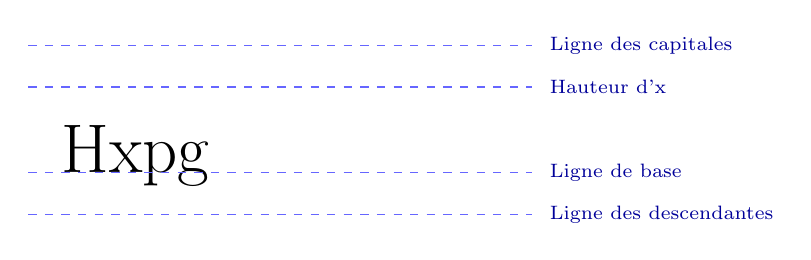
\begin{tikzpicture}
\node[anchor=base west,font=\fontsize{70}{70}\selectfont] at (0,0) {Hxpg};
\foreach \y/\n in {0pt/Ligne de base,31pt/Hauteur d'x,46pt/Ligne des capitales,-15pt/Ligne des descendantes}{
  \draw[blue!60,dashed] (-0.3,\y) -- (6.1,\y);
  \node[anchor=west,font=\scriptsize,blue!60!black] at (6.2,\y) {\n};}
\end{tikzpicture}
\caption{Lignes de repère d'un caractère (positions indicatives).}
\end{figure}

\subsubsection{La ligne de base}

La \terme{ligne de base} (ou \emph{baseline}) est la ligne sur laquelle reposent les lettres. C'est la référence principale pour l'alignement.

\subsubsection{La ligne des capitales}

La \terme{ligne des capitales} (ou \emph{cap height}) est la hauteur des lettres majuscules.

\subsubsection{La ligne des ascendantes}

La \terme{ligne des ascendantes} (ou \emph{ascender line}) est la hauteur des lettres qui montent au-dessus de la hauteur d'x (comme le « b », le « d », le « h », le « k », le « l »).

\subsubsection{La ligne des descendantes}

La \terme{ligne des descendantes} (ou \emph{descender line}) est la ligne sous laquelle descendent certaines lettres (comme le « g », le « j », le « p », le « q », le « y »).

\subsubsection{La hauteur d'x}

La \terme{hauteur d'x} (ou \emph{x-height}) est la hauteur des lettres minuscules sans ascendante ni descendante (comme le « a », le « c », le « e », le « m », le « n », le « o », le « r », le « s », le « u », le « v », le « w », le « x », le « z »).

\subsection{Le rôle de la hauteur d'x}

La \terme{hauteur d'x} est un paramètre important : elle détermine la lisibilité d'une police. Une police avec une grande hauteur d'x est plus lisible en petit corps ; une police avec une petite hauteur d'x est plus élégante en grand corps.

\subsection{Les proportions}

Les caractères ont des proportions différentes :

\begin{itemize}
    \item \terme{Étroits} : caractères condensés.
    \item \terme{Larges} : caractères étendus.
    \item \terme{Normaux} : caractères de proportion standard.
\end{itemize}

Ces proportions influencent la lisibilité et l'expressivité.

\subsection*{Conclusion de la section}

\begin{retenir}
L'\terme{anatomie des caractères} étudie les différentes parties qui composent une lettre : fût, délié, barre, panse, contre-poinçon, empattement, crochet, jambe, bras, queue, épaule, œil, bec. Elle repose sur des \terme{lignes de repère} : ligne de base, ligne des capitales, ligne des ascendantes, ligne des descendantes, hauteur d'x. Ces notions permettent d'identifier, de classer et de choisir les polices.
\end{retenir}

Maintenant que nous connaissons l'anatomie des caractères, nous allons, dans la section suivante, étudier les \terme{grandes familles de polices}.

% ============================================================
\section{Les grandes familles de polices}
% ============================================================

\subsection{Qu'est-ce qu'une famille de polices ?}

\begin{quote}
\textbf{Une famille de polices est un ensemble de caractères qui partagent des caractéristiques communes de style, de proportions et de dessin.}
\end{quote}

On distingue plusieurs grandes familles, classées selon des critères historiques et formels.

\subsection{Les grandes familles}

\subsubsection{Les caractères à empattements (serif)}

Les caractères \terme{à empattements} (ou \emph{serif}) sont terminés par de petits traits appelés empattements. Ils sont considérés comme classiques, élégants, traditionnels.

Sous-catégories :

\begin{itemize}
    \item \terme{Old Style} (Garamond, Jenson) : empattements fins, contraste modéré.
    \item \terme{Transitional} (Baskerville, Times) : contraste plus marqué.
    \item \terme{Modern} (Bodoni, Didot) : contraste très élevé, empattements fins.
    \item \terme{Égyptiens} (Rockwell, Courier) : empattements épais, contraste faible.
\end{itemize}

\subsubsection{Les caractères sans empattements (sans-serif)}

Les caractères \terme{sans empattements} (ou \emph{sans-serif}, \emph{grotesques}) n'ont pas d'empattements. Ils sont considérés comme modernes, fonctionnels, lisibles.

Sous-catégories :

\begin{itemize}
    \item \terme{Grotesques} (Helvetica, Arial) : formes neutres, lisibilité élevée.
    \item \terme{Néo-grotesques} (Univers, Frutiger) : formes plus régulières.
    \item \terme{Géométriques} (Futura, Avant Garde) : formes géométriques (cercle, carré).
    \item \terme{Humanistes} (Gill Sans, Myriad) : formes inspirées de l'écriture.
\end{itemize}

\subsubsection{Les caractères manuscrits (script)}

Les caractères \terme{manuscrits} (ou \emph{script}) imitent l'écriture manuscrite. Ils sont élégants, personnels, décoratifs.

Sous-catégories :

\begin{itemize}
    \item \terme{Calligraphiques} : imitent la calligraphie.
    \item \terme{Manuscrits formels} : imitent l'écriture à la plume.
    \item \terme{Manuscrits informels} : imitent l'écriture rapide.
\end{itemize}

\subsubsection{Les caractères décoratifs (display)}

Les caractères \terme{décoratifs} (ou \emph{display}) sont conçus pour attirer l'attention. Ils sont souvent utilisés pour les titres, les logos, les affiches.

Sous-catégories :

\begin{itemize}
    \item \terme{Fantaisie} : formes originales, inventives.
    \item \terme{Historiques} : imitent des styles anciens.
    \item \terme{Expérimentaux} : formes inédites.
\end{itemize}

\subsubsection{Les caractères à chasse fixe (monospace)}

Les caractères \terme{à chasse fixe} (ou \emph{monospace}) ont des lettres de largeur identique. Ils sont utilisés pour le code, les tableaux, parfois les interfaces.

Exemples : Courier, Consolas, Roboto Mono.

\subsection{Tableau récapitulatif}

\begin{table}[h!]
\centering
\begin{tabular}{@{}lll@{}}
\toprule
\textbf{Famille} & \textbf{Caractéristiques} & \textbf{Exemples} \\
\midrule
Serif & Empattements, classique & Garamond, Times, Bodoni \\
Sans-serif & Sans empattements, moderne & Helvetica, Arial, Futura \\
Script & Manuscrite, élégante & Edwardian Script, Pacifico \\
Display & Décorative, expressive & Impact, Lobster \\
Monospace & Chasse fixe, technique & Courier, Consolas \\
\bottomrule
\end{tabular}
\caption{Les grandes familles de polices.}
\end{table}

\subsection{Choisir une famille}

Le choix d'une famille dépend de :

\begin{itemize}
    \item Du \terme{message} : un message sérieux appelle un serif ou un sans-serif neutre ; un message ludique appelle un display ou un script.
    \item Du \terme{support} : l'impression supporte mieux les serifs fins ; l'écran préfère les sans-serif.
    \item Du \terme{public} : un public âgé préfère les polices lisibles ; un public jeune apprécie les polices originales.
    \item De l'\terme{identité} : une marque de luxe préfère un serif élégant ; une marque technologique préfère un sans-serif moderne.
\end{itemize}

\subsection*{Conclusion de la section}

\begin{retenir}
Les grandes familles de polices sont : les \terme{à empattements} (serif), les \terme{sans empattements} (sans-serif), les \terme{manuscrites} (script), les \terme{décoratives} (display) et les \terme{à chasse fixe} (monospace). Chaque famille a ses caractéristiques, ses usages, ses exemples. Le choix d'une famille dépend du message, du support, du public et de l'identité.
\end{retenir}

Maintenant que nous connaissons les familles de polices, nous allons, dans la section suivante, approfondir la distinction entre \terme{polices avec empattements et sans empattements}.

% ============================================================
\section{Les polices avec empattements et sans empattements}
% ============================================================

\subsection{Les polices avec empattements (serif)}

\subsubsection{Définition}

Les polices \terme{avec empattements} sont terminées par de petits traits appelés empattements. Ces traits peuvent être fins ou épais, droits ou courbes.

\subsubsection{Caractéristiques}

\begin{itemize}
    \item \terme{Classiques} : elles évoquent la tradition, le sérieux, l'élégance.
    \item \terme{Lisibles en petit corps} : les empattements guident l'œil le long de la ligne.
    \item \terme{Contraste} : les pleins et les déliés sont souvent contrastés.
    \item \terme{Expressives} : elles transmettent une ambiance, une époque.
\end{itemize}

\subsubsection{Usages}

\begin{itemize}
    \item \terme{Presse écrite} : journaux, magazines (Times, Garamond).
    \item \terme{Livres} : romans, essais (Garamond, Baskerville).
    \item \terme{Identités} : marques de luxe, institutions (Bodoni, Didot).
    \item \terme{Titres} : titres élégants, traditionnels.
\end{itemize}

\subsubsection{Exemples}

\begin{itemize}
    \item \terme{Garamond} : élégant, lisible, intemporel.
    \item \terme{Baskerville} : contraste marqué, raffiné.
    \item \terme{Bodoni} : contraste très élevé, luxueux.
    \item \terme{Times} : lisible, classique, universel.
\end{itemize}

\subsection{Les polices sans empattements (sans-serif)}

\subsubsection{Définition}

Les polices \terme{sans empattements} n'ont pas d'empattements. Les fûts se terminent par des traits droits ou légèrement arrondis.

\subsubsection{Caractéristiques}

\begin{itemize}
    \item \terme{Modernes} : elles évoquent la modernité, la simplicité, la fonctionnalité.
    \item \terme{Lisibles à l'écran} : leur simplicité les rend adaptées aux écrans.
    \item \terme{Neutres} : elles sont souvent moins expressives que les serifs.
    \item \terme{Variées} : il existe de nombreuses sous-familles (grotesques, géométriques, humanistes).
\end{itemize}

\subsubsection{Usages}

\begin{itemize}
    \item \terme{Web} : sites, applications, interfaces.
    \item \terme{Signalétique} : panneaux, transports, espaces publics.
    \item \terme{Identités} : marques modernes, technologiques.
    \item \terme{Titres} : titres modernes, dynamiques.
\end{itemize}

\subsubsection{Exemples}

\begin{itemize}
    \item \terme{Helvetica} : neutre, universel, intemporel.
    \item \terme{Arial} : lisible, standard, répandu.
    \item \terme{Futura} : géométrique, moderne, élégant.
    \item \terme{Frutiger} : lisible, humaniste, chaleureux.
\end{itemize}

\subsection{Comparaison serif / sans-serif}

\begin{table}[h!]
\centering
\begin{tabular}{@{}lll@{}}
\toprule
\textbf{Critère} & \textbf{Serif} & \textbf{Sans-serif} \\
\midrule
Empattements & Oui & Non \\
Évocation & Tradition, élégance & Modernité, fonctionnalité \\
Lisibilité papier & Excellente & Bonne \\
Lisibilité écran & Moyenne & Excellente \\
Contraste & Souvent élevé & Souvent faible \\
Expressivité & Élevée & Neutre \\
Usages & Presse, livres, luxe & Web, signalétique, tech \\
\bottomrule
\end{tabular}
\caption{Comparaison serif / sans-serif.}
\end{table}

\subsection{Quand utiliser serif ou sans-serif ?}

\subsubsection{Pour le texte courant}

\begin{itemize}
    \item \terme{Papier} : serif (plus lisible en petit corps).
    \item \terme{Écran} : sans-serif (plus lisible en basse résolution).
\end{itemize}

\subsubsection{Pour les titres}

\begin{itemize}
    \item \terme{Serif} : titres élégants, traditionnels.
    \item \terme{Sans-serif} : titres modernes, dynamiques.
\end{itemize}

\subsubsection{Pour les identités}

\begin{itemize}
    \item \terme{Serif} : luxe, tradition, institution.
    \item \terme{Sans-serif} : modernité, technologie, jeunesse.
\end{itemize}

\subsection*{Conclusion de la section}

\begin{retenir}
Les polices \terme{avec empattements} (serif) évoquent la tradition, l'élégance, le sérieux. Les polices \terme{sans empattements} (sans-serif) évoquent la modernité, la simplicité, la fonctionnalité. Le choix entre les deux dépend du support (papier ou écran), du message et de l'identité. En pratique, on utilise souvent les deux : un serif pour le texte courant, un sans-serif pour les titres, ou inversement.
\end{retenir}

Maintenant que nous connaissons la distinction serif/sans-serif, nous allons, dans la section suivante, étudier les \terme{polices manuscrites et décoratives}.

% ============================================================
\section{Les polices manuscrites et décoratives}
% ============================================================

\subsection{Les polices manuscrites (script)}

\subsubsection{Définition}

Les polices \terme{manuscrites} (ou \emph{script}) imitent l'écriture manuscrite. Elles peuvent être calligraphiques, formelles ou informelles.

\subsubsection{Caractéristiques}

\begin{itemize}
    \item \terme{Élégantes} : elles évoquent la finesse, la personnalité.
    \item \terme{Expressives} : elles transmettent une émotion, une ambiance.
    \item \terme{Peu lisibles} : elles sont souvent difficiles à lire en petit corps.
    \item \terme{Décoratives} : elles attirent l'attention.
\end{itemize}

\subsubsection{Usages}

\begin{itemize}
    \item \terme{Invitations} : mariages, événements.
    \item \terme{Logos} : marques élégantes, artisanales.
    \item \terme{Titres} : titres expressifs, poétiques.
    \item \terme{Publicités} : publicités de luxe, de cosmétiques.
\end{itemize}

\subsubsection{Exemples}

\begin{itemize}
    \item \terme{Edwardian Script} : calligraphique, élégante.
    \item \terme{Pacifico} : manuscrite, décontractée.
    \item \terme{Dancing Script} : manuscrite, fluide.
    \item \terme{Great Vibes} : calligraphique, raffinée.
\end{itemize}

\subsection{Les polices décoratives (display)}

\subsubsection{Définition}

Les polices \terme{décoratives} (ou \emph{display}) sont conçues pour attirer l'attention. Elles ont des formes originales, souvent très expressives.

\subsubsection{Caractéristiques}

\begin{itemize}
    \item \terme{Originales} : elles se distinguent des polices classiques.
    \item \terme{Expressives} : elles transmettent une ambiance forte.
    \item \terme{Peu lisibles} : elles ne conviennent pas au texte courant.
    \item \terme{Situationnelles} : elles conviennent à des usages spécifiques.
\end{itemize}

\subsubsection{Usages}

\begin{itemize}
    \item \terme{Titres} : titres d'affiches, de couvertures.
    \item \terme{Logos} : logos originaux, mémorables.
    \item \terme{Publicités} : publicités créatives.
    \item \terme{Événements} : festivals, concerts, fêtes.
\end{itemize}

\subsubsection{Exemples}

\begin{itemize}
    \item \terme{Impact} : massive, percutante.
    \item \terme{Lobster} : rétro, chaleureuse.
    \item \terme{Bebas Neue} : condensée, moderne.
    \item \terme{Cooper Black} : ronde, sympathique.
\end{itemize}

\subsection{Précautions d'usage}

Les polices manuscrites et décoratives sont puissantes mais délicates. Voici quelques précautions :

\begin{itemize}
    \item \terme{Ne pas les utiliser pour le texte courant} : elles sont peu lisibles.
    \item \terme{Ne pas les mélanger} : une seule police décorative par composition.
    \item \terme{Ne pas les surexploiter} : elles perdent leur impact si elles sont partout.
    \item \terme{Vérifier la lisibilité} : tester la police en petit corps, en grand corps, en contexte.
\end{itemize}

\subsection*{Conclusion de la section}

\begin{retenir}
Les polices \terme{manuscrites} (script) imitent l'écriture manuscrite : elles sont élégantes, expressives, mais peu lisibles en petit corps. Les polices \terme{décoratives} (display) sont conçues pour attirer l'attention : elles sont originales, expressives, mais réservées aux titres. Ces polices doivent être utilisées avec précaution : une seule par composition, jamais pour le texte courant.
\end{retenir}

Maintenant que nous connaissons les différentes familles de polices, nous allons, dans la section suivante, étudier la \terme{lisibilité et la facilité de lecture}.

% ============================================================
\section{La lisibilité et la facilité de lecture}
% ============================================================

\subsection{Lisibilité et facilité de lecture : deux notions distinctes}

\subsubsection{La lisibilité}

La \terme{lisibilité} est la qualité d'un caractère ou d'un texte qui le rend identifiable et déchiffrable. Elle dépend des caractéristiques de la police (forme, taille, contraste) et du support (papier, écran).

\subsubsection{La facilité de lecture}

La \terme{facilité de lecture} (ou \emph{readability}) est la qualité d'un texte qui le rend agréable et aisé à lire. Elle dépend de la mise en page (longueur des lignes, interlignage, alignement), du contenu et du contexte.

Un texte peut être \terme{lisible} (on peut déchiffrer chaque mot) mais \terme{difficile à lire} (on se fatigue rapidement). L'objectif est d'atteindre les deux.

\subsection{Les facteurs de lisibilité}

\subsubsection{La forme des caractères}

\begin{itemize}
    \item Les caractères à empattements sont souvent plus lisibles en petit corps.
    \item Les caractères sans empattements sont souvent plus lisibles à l'écran.
    \item Les caractères trop fins ou trop gras sont moins lisibles.
\end{itemize}

\subsubsection{La taille}

\begin{itemize}
    \item \terme{Papier} : 9 à 12 points pour le texte courant.
    \item \terme{Écran} : 14 à 18 pixels pour le texte courant.
    \item \terme{Titres} : 18 points et plus.
\end{itemize}

\subsubsection{Le contraste}

\begin{itemize}
    \item Le texte doit contraster avec le fond.
    \item Le contraste de valeur (clair/foncé) est le plus important.
    \item Éviter les contrastes de couleur trop faibles.
\end{itemize}

\subsubsection{La longueur des lignes}

\begin{itemize}
    \item \terme{Idéal} : 45 à 75 caractères par ligne.
    \item \terme{Trop court} : l'œil doit revenir souvent à la ligne.
    \item \terme{Trop long} : l'œil perd la ligne suivante.
\end{itemize}

\subsubsection{L'interlignage}

\begin{itemize}
    \item \terme{Idéal} : 120\% à 150\% de la taille du texte.
    \item \terme{Trop serré} : le texte est compact, difficile à lire.
    \item \terme{Trop large} : les lignes sont dispersées, la lecture est hachée.
\end{itemize}

\subsubsection{L'alignement}

\begin{itemize}
    \item \terme{Aligné à gauche} : le plus lisible, recommandé pour les textes longs.
    \item \terme{Justifié} : élégant, mais peut créer des espaces irréguliers.
    \item \terme{Centré} : convient aux titres, pas aux textes longs.
    \item \terme{Aligné à droite} : rare, convient à des usages spécifiques.
\end{itemize}

\subsection{Les facteurs de facilité de lecture}

\subsubsection{La structure}

\begin{itemize}
    \item Utiliser des titres, des sous-titres, des paragraphes.
    \item Créer une hiérarchie claire.
    \item Aérer le texte.
\end{itemize}

\subsubsection{Le contenu}

\begin{itemize}
    \item Phrases courtes.
    \item Vocabulaire adapté au public.
    \item Idées organisées logiquement.
\end{itemize}

\subsubsection{Le contexte}

\begin{itemize}
    \item Le texte doit être adapté au support (papier, écran).
    \item Le texte doit être adapté au public (âge, culture).
    \item Le texte doit être adapté à l'usage (lecture rapide, lecture approfondie).
\end{itemize}

\subsection{Tester la lisibilité}

Pour tester la lisibilité d'un texte :

\begin{itemize}
    \item \terme{Imprimer} le texte et le lire à voix haute.
    \item \terme{Zoomer} et \terme{dézoomer} pour vérifier la lisibilité à différentes tailles.
    \item \terme{Demander} à quelqu'un d'autre de le lire.
    \item \terme{Comparer} avec des textes de référence.
\end{itemize}

\subsection*{Conclusion de la section}

\begin{retenir}
La \terme{lisibilité} est la qualité qui rend un texte déchiffrable ; la \terme{facilité de lecture} est la qualité qui rend un texte agréable à lire. Les facteurs de lisibilité sont : la forme des caractères, la taille, le contraste, la longueur des lignes, l'interlignage, l'alignement. Les facteurs de facilité de lecture sont : la structure, le contenu, le contexte. Un designer doit viser les deux.
\end{retenir}

Maintenant que nous savons ce qui rend un texte lisible, nous allons, dans la section suivante, étudier la \terme{taille des caractères et les unités typographiques}.

% ============================================================
\section{La taille des caractères et les unités typographiques}
% ============================================================

\subsection{Les unités typographiques}

\subsubsection{Le point}

Le \terme{point} (pt) est l'unité de mesure traditionnelle de la typographie. Il vaut environ 1/72 de pouce, soit 0,353 mm.

\begin{itemize}
    \item \terme{Point Didot} : 0,376 mm (utilisé en Europe).
    \item \terme{Point pica} : 0,353 mm (utilisé aux États-Unis).
\end{itemize}

\subsubsection{Le pica}

Le \terme{pica} vaut 12 points, soit environ 4,23 mm. Il est utilisé pour les mesures de colonnes, de marges, d'espacements.

\subsubsection{Le pixel}

Le \terme{pixel} (px) est l'unité de mesure des écrans. Il correspond à un point de l'image numérique.

\subsubsection{Le em}

Le \terme{em} est une unité relative : il correspond à la taille de la police. Un em = la taille du caractère. Il est utilisé pour les espacements, les marges, les largeurs.

\subsubsection{Le rem}

Le \terme{rem} (root em) est une unité relative à la taille de la police racine (généralement 16 px sur le web).

\subsubsection{Le pourcentage}

Le \terme{pourcentage} (\%) est une unité relative, souvent utilisée pour les largeurs et les hauteurs.

\subsection{Correspondances approximatives}

\begin{table}[h!]
\centering
\begin{tabular}{@{}ll@{}}
\toprule
\textbf{Unité} & \textbf{Équivalence} \\
\midrule
1 point & 0,353 mm \\
1 pica & 12 points \\
1 pouce & 72 points \\
1 pixel & 1/96 pouce (standard web) \\
1 em & Taille de la police \\
\bottomrule
\end{tabular}
\caption{Correspondances entre unités typographiques.}
\end{table}

\subsection{Choisir la taille}

\subsubsection{Texte courant}

\begin{itemize}
    \item \terme{Papier} : 9 à 12 points.
    \item \terme{Écran} : 14 à 18 pixels.
    \item \terme{Mobile} : 16 pixels minimum.
\end{itemize}

\subsubsection{Titres}

\begin{itemize}
    \item \terme{Titre principal} : 24 à 72 points.
    \item \terme{Sous-titre} : 16 à 24 points.
    \item \terme{Titre de section} : 18 à 36 points.
\end{itemize}

\subsubsection{Légendes et mentions}

\begin{itemize}
    \item \terme{Légendes} : 8 à 10 points.
    \item \terme{Mentions légales} : 6 à 8 points.
\end{itemize}

\subsection{La hiérarchie des tailles}

La hiérarchie des tailles doit être \terme{proportionnée}. On utilise souvent une échelle :

\begin{itemize}
    \item \terme{Échelle 1,25} : chaque taille est 1,25 fois plus grande que la précédente.
    \item \terme{Échelle 1,5} : chaque taille est 1,5 fois plus grande.
    \item \terme{Échelle 2} : chaque taille est 2 fois plus grande.
\end{itemize}

Ces échelles permettent de créer une hiérarchie cohérente.

\subsection*{Conclusion de la section}

\begin{retenir}
Les \terme{unités typographiques} sont : le point (pt), le pica, le pixel (px), le em, le rem, le pourcentage. Le choix de la taille dépend du support, du public et du type de texte. La hiérarchie des tailles doit être proportionnée, souvent basée sur une échelle (1,25, 1,5, 2).
\end{retenir}

Maintenant que nous connaissons les unités typographiques, nous allons, dans la section suivante, étudier l'\terme{interlignage, le crénage et l'approche}.

% ============================================================
\section{L'interlignage, le crénage et l'approche}
% ============================================================

\subsection{L'interlignage}

\subsubsection{Définition}

L'\terme{interlignage} (ou \emph{leading}) est l'espace vertical entre les lignes de texte. Il se mesure de ligne de base à ligne de base.

\subsubsection{Unités}

L'interlignage se mesure en points, en pixels, en em ou en pourcentage.

\subsubsection{Valeurs recommandées}

\begin{itemize}
    \item \terme{Texte courant} : 120\% à 150\% de la taille du texte.
    \item \terme{Titres} : 100\% à 120\%.
    \item \terme{Petits textes} : 130\% à 160\%.
\end{itemize}

\subsubsection{Effets}

\begin{itemize}
    \item \terme{Interlignage serré} : le texte est compact, dense. Convient aux titres.
    \item \terme{Interlignage normal} : le texte est lisible, aéré. Convient au texte courant.
    \item \terme{Interlignage large} : le texte est dispersé, aéré. Convient aux textes courts, aux citations.
\end{itemize}

\subsection{Le crénage}

\subsubsection{Définition}

Le \terme{crénage} (ou \emph{kerning}) est l'ajustement de l'espace entre deux caractères spécifiques. Il permet de corriger les espacements irréguliers.

\subsubsection{Pourquoi ajuster le crénage ?}

Certaines paires de lettres créent des espacements visuellement irréguliers :

\begin{itemize}
    \item \terme{AV} : espace trop large.
    \item \terme{To} : espace trop large.
    \item \terme{WA} : espace trop large.
    \item \terme{fi} : espace trop serré.
\end{itemize}

L'ajustement du crénage permet d'obtenir un espacement régulier.

\subsubsection{Comment ajuster ?}

Dans les logiciels, on peut :

\begin{itemize}
    \item Utiliser le \terme{crénage automatique} (métriques de la police).
    \item Utiliser le \terme{crénage optique} (ajustement automatique).
    \item Ajuster \terme{manuellement} (pour les titres, les logos).
\end{itemize}

\subsection{L'approche}

\subsubsection{Définition}

L'\terme{approche} (ou \emph{tracking}) est l'ajustement global de l'espace entre tous les caractères d'un texte. Contrairement au crénage, qui agit sur des paires spécifiques, l'approche agit sur l'ensemble.

\subsubsection{Unités}

L'approche se mesure en millièmes d'em (par exemple, 0, -10, +50).

\subsubsection{Effets}

\begin{itemize}
    \item \terme{Approche négative} : les caractères sont rapprochés. Convient aux titres.
    \item \terme{Approche positive} : les caractères sont espacés. Convient aux petits textes, aux majuscules.
\end{itemize}

\subsection{Interlignage, crénage, approche : différences}

\begin{table}[h!]
\centering
\begin{tabular}{@{}lll@{}}
\toprule
\textbf{Terme} & \textbf{Portée} & \textbf{Dimension} \\
\midrule
Interlignage & Lignes & Verticale \\
Crénage & Paires de caractères & Horizontale \\
Approche & Tous les caractères & Horizontale \\
\bottomrule
\end{tabular}
\caption{Différences entre interlignage, crénage et approche.}
\end{table}

\subsection{Applications}

\subsubsection{Pour les titres}

\begin{itemize}
    \item \terme{Interlignage} : serré (100\% à 120\%).
    \item \terme{Crénage} : ajusté manuellement.
    \item \terme{Approche} : négative (légèrement).
\end{itemize}

\subsubsection{Pour le texte courant}

\begin{itemize}
    \item \terme{Interlignage} : 120\% à 150\%.
    \item \terme{Crénage} : automatique.
    \item \terme{Approche} : 0.
\end{itemize}

\subsubsection{Pour les logos}

\begin{itemize}
    \item \terme{Interlignage} : ajusté visuellement.
    \item \terme{Crénage} : ajusté caractère par caractère.
    \item \terme{Approche} : ajustée globalement.
\end{itemize}

\subsection*{Conclusion de la section}

\begin{retenir}
L'\terme{interlignage} est l'espace vertical entre les lignes. Le \terme{crénage} est l'espace entre deux caractères spécifiques. L'\terme{approche} est l'espace global entre tous les caractères. Ces trois paramètres sont essentiels pour la lisibilité et l'esthétique d'un texte. Ils doivent être ajustés selon le type de texte et le contexte.
\end{retenir}

Maintenant que nous maîtrisons les espacements, nous allons, dans la section suivante, étudier l'\terme{association des polices}.

% ============================================================
\section{L'association des polices}
% ============================================================

\subsection{Pourquoi associer des polices ?}

L'association de polices permet de :

\begin{itemize}
    \item \terme{Créer une hiérarchie} : distinguer les titres du texte courant.
    \item \terme{Créer du contraste} : opposer des styles différents.
    \item \terme{Enrichir} la composition : varier les formes, les ambiances.
    \item \terme{Exprimer} une identité : associer des polices caractéristiques.
\end{itemize}

Mais l'association de polices est délicate : mal faite, elle crée de la confusion.

\subsection{Les principes d'association}

\subsubsection{Principe 1 : Limiter le nombre de polices}

\begin{itemize}
    \item \terme{Idéal} : 1 à 2 polices.
    \item \terme{Maximum} : 3 polices (dans des cas spécifiques).
    \item \terme{Éviter} : plus de 3 polices, sauf projet exceptionnel.
\end{itemize}

\subsubsection{Principe 2 : Créer du contraste}

Les polices associées doivent être \terme{suffisamment différentes} pour créer du contraste, mais \terme{suffisamment proches} pour ne pas se heurter.

\begin{itemize}
    \item \terme{Bon contraste} : serif + sans-serif.
    \item \terme{Bon contraste} : condensé + large.
    \item \terme{Bon contraste} : classique + moderne.
    \item \terme{Mauvais contraste} : deux serifs similaires.
    \item \terme{Mauvais contraste} : deux sans-serif similaires.
\end{itemize}

\subsubsection{Principe 3 : Chercher l'harmonie}

Les polices associées doivent \terme{s'harmoniser} : elles doivent avoir des proportions compatibles, des hauteurs d'x proches, des styles cohérents.

\subsubsection{Principe 4 : Définir les rôles}

Chaque police doit avoir un \terme{rôle} :

\begin{itemize}
    \item \terme{Police de titre} : pour les titres, les accroches.
    \item \terme{Police de texte} : pour le texte courant.
    \item \terme{Police d'accent} : pour les citations, les légendes.
\end{itemize}

\subsection{Les associations classiques}

\subsubsection{Serif + sans-serif}

Association la plus courante : un serif pour le texte, un sans-serif pour les titres (ou inversement).

Exemples :
\begin{itemize}
    \item \terme{Garamond + Helvetica} : élégant et moderne.
    \item \terme{Times + Arial} : classique et neutre.
    \item \terme{Bodoni + Futura} : luxueux et géométrique.
\end{itemize}

\subsubsection{Sans-serif + sans-serif}

Association plus délicate : il faut choisir des sans-serif suffisamment différents.

Exemples :
\begin{itemize}
    \item \terme{Helvetica + Futura} : neutre et géométrique.
    \item \terme{Roboto + Montserrat} : moderne et élégant.
\end{itemize}

\subsubsection{Serif + serif}

Association difficile : il faut choisir des serifs très différents.

Exemples :
\begin{itemize}
    \item \terme{Garamond + Bodoni} : ancien et moderne.
    \item \terme{Times + Rockwell} : classique et égyptien.
\end{itemize}

\subsubsection{Avec une police décorative}

Une police décorative peut être associée à une police neutre.

Exemples :
\begin{itemize}
    \item \terme{Lobster + Lato} : décoratif et neutre.
    \item \terme{Pacifico + Open Sans} : manuscrit et lisible.
\end{itemize}

\subsection{Les erreurs d'association}

\begin{itemize}
    \item \terme{Trop de polices} : plus de 3 polices créent la confusion.
    \item \terme{Polices trop similaires} : deux serifs similaires créent un conflit.
    \item \terme{Polices trop différentes} : deux polices sans rapport créent un choc.
    \item \terme{Pas de rôles définis} : les polices sont utilisées au hasard.
    \item \terme{Polices inadaptées au message} : les polices ne correspondent pas à l'ambiance.
\end{itemize}

\subsection*{Conclusion de la section}

\begin{retenir}
L'\terme{association des polices} permet de créer une hiérarchie, du contraste, de l'enrichissement. Les principes sont : limiter le nombre de polices (1 à 2 idéalement), créer du contraste, chercher l'harmonie, définir les rôles. Les associations classiques sont : serif + sans-serif, sans-serif + sans-serif, serif + serif, avec une police décorative. Les erreurs courantes sont : trop de polices, polices trop similaires, polices trop différentes, pas de rôles définis, polices inadaptées.
\end{retenir}

Maintenant que nous savons associer les polices, nous allons, dans la section suivante, étudier la \terme{hiérarchie typographique}.

% ============================================================
\section{La hiérarchie typographique}
% ============================================================

\subsection{Qu'est-ce que la hiérarchie typographique ?}

\begin{quote}
\textbf{La hiérarchie typographique est l'organisation des différents niveaux de texte d'une composition, selon leur importance, de manière à guider le regard du lecteur.}
\end{quote}

La hiérarchie typographique est essentielle : elle permet au lecteur d'identifier immédiatement le message principal, puis les messages secondaires, puis les informations pratiques.

\subsection{Les niveaux de hiérarchie}

On distingue généralement 3 à 5 niveaux :

\begin{enumerate}
    \item \terme{Titre principal} (ou \emph{titre de niveau 1}) : le plus important.
    \item \terme{Sous-titre} (ou \emph{titre de niveau 2}) : secondaire.
    \item \terme{Titre de section} (ou \emph{titre de niveau 3}) : tertiaire.
    \item \terme{Chapô} : introduction, résumé.
    \item \terme{Texte courant} : le corps du texte.
    \item \terme{Légende} : texte accompagnant une image.
    \item \terme{Mention} : informations techniques.
\end{enumerate}

\subsection{Les moyens de créer la hiérarchie}

\subsubsection{La taille}

Plus un texte est grand, plus il est important.

\subsubsection{La graisse}

Plus un texte est gras, plus il est important.

\subsubsection{La couleur}

Les couleurs vives attirent plus que les couleurs neutres.

\subsubsection{La police}

Changer de police crée une distinction.

\subsubsection{La casse}

Les majuscules attirent plus que les minuscules.

\subsubsection{Le style}

Italique, souligné, exposant, etc.

\subsubsection{La position}

Les éléments en haut, au centre, à gauche sont vus en premier.

\subsubsection{L'espacement}

Un élément isolé par du vide attire plus.

\subsection{Construire une hiérarchie}

Pour construire une hiérarchie typographique, on peut suivre cette méthode :

\begin{enumerate}
    \item \terme{Identifier les niveaux} : quels sont les niveaux de texte ?
    \item \terme{Définir les rôles} : quelle police pour quel niveau ?
    \item \terme{Définir les tailles} : quelle taille pour chaque niveau ?
    \item \terme{Définir les graisses} : quelle graisse pour chaque niveau ?
    \item \terme{Définir les couleurs} : quelle couleur pour chaque niveau ?
    \item \terme{Tester} : vérifier la hiérarchie sur différents supports.
\end{enumerate}

\subsection{Exemple de hiérarchie}

Prenons une affiche de concert :

\begin{itemize}
    \item \terme{Nom du groupe} : 72 pt, gras, noir.
    \item \terme{Date et lieu} : 24 pt, normal, rouge.
    \item \terme{Description} : 14 pt, normal, gris.
    \item \terme{Mentions légales} : 8 pt, normal, gris clair.
\end{itemize}

Cette hiérarchie guide le regard du nom du groupe (le plus important) vers les mentions légales (le moins important).

\subsection{La hiérarchie et la composition}

La hiérarchie typographique s'intègre dans la composition générale. Elle doit respecter :

\begin{itemize}
    \item L'\terme{équilibre} : les masses de texte sont équilibrées.
    \item L'\terme{alignement} : les textes sont alignés.
    \item La \terme{proximité} : les textes liés sont proches.
    \item Le \terme{contraste} : les textes contrastent.
    \item L'\terme{espace négatif} : les textes respirent.
\end{itemize}

\subsection{Les erreurs de hiérarchie typographique}

\begin{itemize}
    \item \terme{Pas de hiérarchie} : tous les textes ont la même taille.
    \item \terme{Hiérarchie inversée} : le texte secondaire est plus grand que le principal.
    \item \terme{Trop de niveaux} : trop de tailles, de graisses, de couleurs.
    \item \terme{Hiérarchie contradictoire} : deux éléments se disputent l'attention.
    \item \terme{Hiérarchie incohérente} : les niveaux ne sont pas respectés.
\end{itemize}

\subsection*{Conclusion de la section}

\begin{retenir}
La \terme{hiérarchie typographique} organise les niveaux de texte selon leur importance. Elle se crée par la taille, la graisse, la couleur, la police, la casse, le style, la position et l'espacement. Elle doit respecter les principes de composition : équilibre, alignement, proximité, contraste, espace négatif. Les erreurs courantes sont : pas de hiérarchie, hiérarchie inversée, trop de niveaux, hiérarchie contradictoire, hiérarchie incohérente.
\end{retenir}

Maintenant que nous maîtrisons la hiérarchie typographique, nous allons, dans la section suivante, étudier la \terme{typographie dans la publicité}.

% ============================================================
\section{La typographie dans la publicité}
% ============================================================

\subsection{Le rôle de la typographie en publicité}

En publicité, la typographie a un rôle spécifique : elle doit \terme{attirer l'attention}, \terme{transmettre un message} et \terme{créer une émotion} en un temps très court. Le spectateur voit une affiche pendant quelques secondes : le message doit être compris immédiatement.

\subsection{Les caractéristiques de la typographie publicitaire}

\subsubsection{Impact}

La typographie publicitaire doit être \terme{impactante} : elle doit attirer l'attention.

\begin{itemize}
    \item Grandes tailles.
    \item Graisses épaisses.
    \item Contrastes forts.
    \item Polices originales.
\end{itemize}

\subsubsection{Clarté}

La typographie publicitaire doit être \terme{claire} : le message doit être compris immédiatement.

\begin{itemize}
    \item Peu de texte.
    \item Hiérarchie évidente.
    \item Lisibilité maximale.
\end{itemize}

\subsubsection{Expressivité}

La typographie publicitaire doit être \terme{expressive} : elle doit transmettre une ambiance, une émotion.

\begin{itemize}
    \item Polices adaptées au message.
    \item Couleurs expressives.
    \item Compositions dynamiques.
\end{itemize}

\subsubsection{Mémorisation}

La typographie publicitaire doit être \terme{mémorisable} : elle doit laisser une trace.

\begin{itemize}
    \item Polices caractéristiques.
    \item Compositions originales.
    \item Slogans typographiques.
\end{itemize}

\subsection{Les types de typographie publicitaire}

\subsubsection{Typographie de marque}

C'est la typographie d'un logo, d'une marque. Elle doit être \terme{unique}, \terme{mémorisable}, \terme{intemporelle}.

Exemples : Coca-Cola, Google, FedEx.

\subsubsection{Typographie de titre}

C'est la typographie d'un titre, d'une accroche. Elle doit être \terme{impactante}, \terme{expressive}, \terme{adaptée au message}.

Exemples : titres d'affiches, titres de publicités.

\subsubsection{Typographie de slogan}

C'est la typographie d'un slogan. Elle doit être \terme{claire}, \terme{mémorisable}, \terme{cohérente avec la marque}.

Exemples : « Just Do It » (Nike), « Think Different » (Apple).

\subsubsection{Typographie d'information}

C'est la typographie des informations pratiques (date, lieu, prix). Elle doit être \terme{lisible}, \terme{discrète}, \terme{cohérente}.

\subsection{Les techniques publicitaires}

\subsubsection{La typographie expressive}

Utiliser la typographie pour exprimer une émotion, une idée.

Exemples :
\begin{itemize}
    \item Un mot qui fond : typographie liquide.
    \item Un mot qui explose : typographie éclatée.
    \item Un mot qui brûle : typographie enflammée.
\end{itemize}

\subsubsection{La typographie image}

Utiliser la typographie comme une image.

Exemples :
\begin{itemize}
    \item Un mot qui forme une image.
    \item Un mot qui remplace une image.
    \item Un mot qui se transforme en image.
\end{itemize}

\subsubsection{La typographie interactive}

Utiliser la typographie de manière interactive.

Exemples :
\begin{itemize}
    \item Un mot qui s'anime.
    \item Un mot qui réagit au survol.
    \item Un mot qui change selon le contexte.
\end{itemize}

\subsection{Les erreurs de typographie publicitaire}

\begin{itemize}
    \item \terme{Trop de texte} : le message est noyé.
    \item \terme{Typographie illisible} : le message n'est pas compris.
    \item \terme{Typographie incohérente} : le message est brouillé.
    \item \terme{Typographie inadaptée} : le message est décalé.
    \item \terme{Typographie sans hiérarchie} : le message est confus.
\end{itemize}

\subsection*{Conclusion de la section}

\begin{retenir}
En publicité, la typographie doit \terme{attirer l'attention}, \terme{transmettre un message} et \terme{créer une émotion} en un temps très court. Elle doit être \terme{impactante}, \terme{claire}, \terme{expressive} et \terme{mémorisable}. Les types de typographie publicitaire sont : typographie de marque, de titre, de slogan, d'information. Les techniques sont : typographie expressive, typographie image, typographie interactive. Les erreurs sont : trop de texte, typographie illisible, incohérente, inadaptée, sans hiérarchie.
\end{retenir}

Maintenant que nous connaissons la typographie publicitaire, nous allons, dans la dernière section de ce chapitre, étudier les \terme{erreurs typographiques à éviter}.

% ============================================================
\section{Les erreurs typographiques à éviter}
% ============================================================

\subsection{Pourquoi étudier les erreurs ?}

Connaître les erreurs typographiques permet de les éviter, de les reconnaître et de les corriger. Cette section présente les erreurs les plus fréquentes.

\subsection{Les erreurs de choix de police}

\subsubsection{Trop de polices}

Utiliser plus de 3 polices crée de la confusion. Il faut limiter à 1 ou 2 polices.

\subsubsection{Polices inadaptées au message}

Utiliser une police décorative pour un texte sérieux, ou une police classique pour un message ludique.

\subsubsection{Polices inadaptées au support}

Utiliser une police avec des empattements fins pour l'écran, ou une police trop large pour un petit format.

\subsubsection{Polices illisibles}

Utiliser une police trop fine, trop grasse, trop condensée, ou trop originale.

\subsection{Les erreurs de taille}

\subsubsection{Texte trop petit}

Un texte trop petit est illisible. Il faut respecter les tailles minimales (9 pt pour le papier, 14 px pour l'écran).

\subsubsection{Texte trop grand}

Un texte trop grand écrase les autres éléments. Il faut proportionner.

\subsubsection{Pas de hiérarchie}

Tous les textes ont la même taille. Il faut créer une hiérarchie.

\subsection{Les erreurs d'espacement}

\subsubsection{Interlignage trop serré}

Le texte est compact, difficile à lire.

\subsubsection{Interlignage trop large}

Les lignes sont dispersées, la lecture est hachée.

\subsubsection{Crénage négligé}

Les espacements entre les lettres sont irréguliers.

\subsubsection{Approche excessive}

Les lettres sont trop espacées ou trop serrées.

\subsection{Les erreurs d'alignement}

\subsubsection{Alignements multiples}

Utiliser trop d'alignements différents dans une même composition.

\subsubsection{Alignements approximatifs}

Les textes sont presque alignés, mais pas tout à fait.

\subsubsection{Centrage excessif}

Centrer tous les textes crée une composition monotone.

\subsection{Les erreurs de couleur}

\subsubsection{Contraste insuffisant}

Un texte gris clair sur fond blanc est illisible.

\subsubsection{Contraste excessif}

Un texte rouge sur fond vert crée une vibration.

\subsubsection{Couleurs incohérentes}

Utiliser trop de couleurs pour le texte.

\subsection{Les erreurs de contenu}

\subsubsection{Fautes d'orthographe}

Les fautes d'orthographe discréditent le message.

\subsubsection{Ve uves et orphelines}

Les veuves (mot seul en fin de paragraphe) et les orphelines (mot seul en début de page) sont inesthétiques.

\subsubsection{Ponctuation incorrecte}

Les espaces avant et après la ponctuation doivent être respectés.

\subsubsection{Majuscules excessives}

Écrire tout en majuscules rend le texte difficile à lire.

\subsection{Les erreurs techniques}

\subsubsection{Polices manquantes}

Ne pas incorporer les polices dans un PDF.

\subsubsection{Polices vectorisées}

Vectoriser le texte le rend non modifiable.

\subsubsection{Polices non libres de droits}

Utiliser une police sans licence.

\subsection{Méthode de correction}

\begin{enumerate}
    \item \terme{Relire} : vérifier l'orthographe, la ponctuation, les espaces.
    \item \terme{Analyser} : identifier les erreurs typographiques.
    \item \terme{Prioriser} : commencer par les plus importantes.
    \item \terme{Corriger} : appliquer les principes.
    \item \terme{Vérifier} : contrôler le résultat.
\end{enumerate}

\subsection*{Conclusion de la section}

\begin{retenir}
Les erreurs typographiques concernent le \terme{choix de police}, la \terme{taille}, l'\terme{espacement}, l'\terme{alignement}, la \terme{couleur}, le \terme{contenu} et la \terme{technique}. Elles peuvent être évitées par la connaissance des principes et corrigées par une méthode structurée.
\end{retenir}

% ============================================================
\section*{Exercices pratiques}
\addcontentsline{toc}{section}{Exercices pratiques}
% ============================================================

\subsubsection*{Exercice 1 --- Hiérarchie typographique (Illustrator)}

Crée une affiche A4 pour un concert fictif avec \emph{trois niveaux} de texte : titre, informations (date, lieu) et mentions secondaires. Utilise au maximum deux polices.

\begin{retenir}
\textbf{Critère de réussite :} en plissant les yeux, on distingue immédiatement les trois niveaux grâce à la taille, à la graisse et à l'espacement, sans changer plus de deux polices.
\end{retenir}

\subsubsection*{Exercice 2 --- Association de polices (Photoshop ou Illustrator)}

Compose le même titre et le même paragraphe avec trois associations différentes : serif + sans-serif, deux sans-serif de graisses contrastées, police display + police neutre. Compare les résultats et justifie ton choix en trois phrases.

\begin{astuce}
Si deux polices se ressemblent sans être identiques, elles se concurrencent : accentue le contraste (taille, graisse, style) ou garde une seule famille.
\end{astuce}

\subsubsection*{Exercice 3 --- Correction d'erreurs typographiques}

Prends un visuel existant (le tien ou une publicité) contenant au moins cinq erreurs typographiques : interlignage, crénage, alignement, contraste, lisibilité. Liste-les, puis corrige-les en suivant la méthode relire, analyser, prioriser, corriger, vérifier.

\begin{retenir}
\textbf{Critère de réussite :} chaque erreur est nommée, la correction est visible en comparant l'avant et l'après, et la lisibilité est contrôlée à taille réduite.
\end{retenir}

% ============================================================
\section*{Conclusion du chapitre}
\addcontentsline{toc}{section}{Conclusion du chapitre}
% ============================================================

Nous voici au terme du chapitre 4. Nous avons parcouru la typographie sous tous ses aspects :

\begin{itemize}
    \item \terme{Définition et histoire} : la typographie est l'art et la technique de la composition des textes.
    \item \terme{Anatomie des caractères} : fût, délié, barre, panse, empattement, etc.
    \item \terme{Grandes familles de polices} : serif, sans-serif, script, display, monospace.
    \item \terme{Serif et sans-serif} : distinction fondamentale.
    \item \terme{Polices manuscrites et décoratives} : usages spécifiques.
    \item \terme{Lisibilité et facilité de lecture} : deux notions distinctes.
    \item \terme{Taille et unités typographiques} : point, pica, pixel, em, rem.
    \item \terme{Interlignage, crénage, approche} : les trois espacements.
    \item \terme{Association des polices} : principes et erreurs.
    \item \terme{Hiérarchie typographique} : organisation des niveaux de texte.
    \item \terme{Typographie publicitaire} : impact, clarté, expressivité, mémorisation.
    \item \terme{Erreurs typographiques} : comment les éviter et les corriger.
\end{itemize}

La typographie est l'un des piliers du design graphique. Elle porte le message verbal, structure la composition, transmet une identité, crée une émotion. Un designer qui maîtrise la typographie dispose d'un levier puissant pour communiquer.

Mais la typographie ne s'utilise pas seule : elle interagit avec les autres éléments de la composition (couleur, image, espace). C'est pourquoi il est essentiel de continuer à pratiquer, à expérimenter, à observer. La théorie est une base, mais c'est la pratique qui fait le designer.

Dans le chapitre suivant, nous étudierons la \terme{culture visuelle et l'analyse graphique}. Nous verrons comment développer son regard, comment analyser une composition, comment construire une bibliothèque de références. Ce sera l'occasion de mettre en pratique tout ce que tu as appris sur la composition, la couleur et la typographie.

\vspace{2em}

\begin{center}
\textit{Fin du chapitre 4 --- Typographie et communication visuelle.}

\vspace{1em}

\textbf{Prochain chapitre : Chapitre 5 --- Culture visuelle et analyse graphique.}
\end{center}